\chapter{Valutazione dell'incertezza di tipo A e B}

\begin{figure}[h]
    \centering
    \includegraphics[scale = 0.5]{Video del bro.jpg}
\end{figure}

\newpage 

\section{Valutazione dell'incertezza}
\footnote{Slide della prof | SDME 2 Incertezza secondo GUM parte II | pag 2 - 5 \\  
Appunti | 2025-03-07 | pag 10 - 11}

Come scritto precedentemente, il problema che si pone nella misura è quello di "riportare" gli strumenti utilizzati in statistica 
in una popolazione con infiniti elementi all'insieme delle misure con elementi finiti. \newline 

Quindi dobbiamo discutere delle stime dei parametri da campioni e non dalla popolazione. \newline 

Si utilizza il valore medio sperimentale $\overline{x}$ perché è la stima migliore del valore atteso della media $\mu$ della popolazione: 
si dice che $\overline{x}$ è il miglior stimatore corretto e consistente di $\mu$. \newline 

\begin{tcolorbox}
    Il concetto di stimatore corretto e consistente non viene approfondito in questo corso, lo diamo per buono
\end{tcolorbox}


Per quanto riguarda lo scarto tipo $\sigma$ della popolazione, 
si parte dall'espressione dello scarto tipo sperimentale: 

{
    \Large 
    \begin{equation}
        s(x_k)
        = 
        \sqrt
        {
            \frac{1}{N-1} \sum_{k = 1}^{N} 
            (x_k - \overline{x})^{2}
        }
    \end{equation}
}

La deviazione standard sperimentale $s(x_k)$ rappresenta il grado di attendibilità della generica misura $x_k$ 
fra le N del campione o, in altri termini, quantifica la dispersione degli N valori misurato attorno al loro valore medio $\overline{x}$. \newline 

Graficando K serie di misura: 

\begin{figure}[h]
    \centering
    \includegraphics[scale = 0.8]{Esempi di serie di misure.PNG}
\end{figure}

si può notare che, in ogni singola serie di misura, quella indicata con la x blu è il risultato della singola misura, 
invece la x in rosso indica il valore medio della singola serie. \newline 

Mettendo le serie insieme, si può calcolare e determinare la dispersione dei valori medi sperimentali (cioè la dispersione delle x rosse). \newline 

Si dimostra (cioè non lo dimostriamo, prendiamolo per buono) che la varianza del valore medio sperimentale fra i vari gruppi di N misure, 
è esprimibile nel seguente modo: 

{
    \Large 
    \begin{equation}
        s^{2} (\overline{x}) 
        = 
        \frac{s^{2} (x_k)}{N}
    \end{equation}
}

allora, con dei semplici passaggi algebrici e sostituzioni: 

{
    \Large 
    \begin{equation}
        \begin{split}
            s(\overline{x})
            &= 
            \frac{s(x_k)}{\sqrt{N}} 
            \\ 
            &= 
            \sqrt
            {
                \frac{1}{N (N-1)}
                \sum_{k = 1}^{N}
                (x_k - \overline{x})^{2}
            }
        \end{split}
    \end{equation}
}

$s(x_k)$ NON è uno stimatore corretto di $\sigma$ e va diviso per $\sqrt{N}$ per diventarlo. \newline 

$s(\overline{x})$, cioè lo scarto tipo del valore medio sperimentale, costituisce una stima della deviazione standard $\sigma$ di tutta la popolazione. \newline 

Quindi useremo: 

\begin{itemize}
    \item $\overline{x}$ al posto di $\mu$ 
    \item $s(\overline{x})$ al posto di $\sigma$
\end{itemize}

\newpage 

\section{Valutazione dell'incertezza di tipo A}
\footnote{Slide della prof | SDME 2 Incertezza secondo GUM parte II | pag 6 \\  
Appunti | 2025-03-07 | pag 12}

La varianza sperimentale della media $s^{2}(\overline{x})$ e lo scarto tipo sperimentale della media $s (\overline{x})$, 
indicano quanto bene $\overline{x}$ stimi il valore medio $\mu$ della popolazione (che sarebbe il valore atteso) e, pertanto, verranno 
adottati come valutazioni quantitative dell'incertezza di $\overline{x}$. \newline 

Diremo quindi che una grandezza fisica X, che è la grandezza sotto misura, determinata con N osservazioni ripetute, 
avrà un'incertezza (uncertainty) sulla stima $\overline{x}$ pari a: 

{
    \Large 
    \begin{equation}
        u^{2} (x) = s^{2} (\overline{x})
    \end{equation}
}

in termini di varianza e 

{
    \Large 
    \begin{equation}
        u(x) = s(\overline{x})
    \end{equation}
}

in termini di scarto tipo. \newline 

Quindi, se avremo a che fare solo con misure di tipo A, 
la misura finale dobbiamo esprimerla come: 

{
    \Large 
    \begin{equation}
        \begin{split}
            X 
            &= 
            \overline{x} \pm u_a (\overline{x}) \text{ } [u.d.m.] 
            \\ 
            &= 
            \overline{x} \pm s (\overline{x}) \text{ } [u.d.m.]  
        \end{split}
    \end{equation}
}

dove: 
\begin{itemize}
    \item X è la grandezza sotto misura
\end{itemize}

\newpage

\section{Valutazione dell'incertezza di tipo B}
\footnote{Slide della prof | SDME 2 Incertezza secondo GUM parte II | pag 7 - 10 \\  
Appunti | 2025-03-07 | pag 12 - 13 | 2025-03-11 | pag 2 - 4}

Adesso passiamo dall'incertezza di tipo A, cioè da misure ripetute, 
all'incertezza di tipo B, cioè una misura da una ripetizione. \newline 

Quando una grandezza X non viene determinata da osservazioni ripetute, 
bensì con una misura singola, 
la varianza stimata $u^{2} (x)$ o lo scarto tipo u(x) sono valutati per mezzo 
di un giudizio scientifico basato su tutte le altre informazioni disponibili: 

\begin{itemize}
    \item dati di misurazioni precedenti 
    \item conoscenza del comportamento e delle proprietà dei materiali e degli strumenti 
    \item specifiche tecniche del costruttore (sono indicate nel manuale dello strumento)
    \item dati forniti in certificato di taratura (quindi dai LAT) 
    \item incertezze assegnate a valori di riferimento presi da manuali 
\end{itemize}

L'uso di tali informazioni, per una valutazione di incertezza di tipo B, 
richiede conoscenza, esperienza e perizia che possono acquisirsi solo con la pratica e col tempo. \newline 

L'analisi statistica sulle misure è un'indagine che viene fatta durante la taratura di uno strumento. \newline 

Il certificato di taratura accompagna il singolo strumento nel suo impiego e chi lo utilizza sa che le indicazioni fornite possono avere 
un'incertezza compresa entro l'intervallo dichiarato sul certificato di taratura, 
con un assegnato livello di confidenza. \newline 

Più spesso, i costruttori di strumentazione assegnano le specifiche di accuratezza con valori numerici valida per tutti gli 
esemplari di un dato modello, e per essi dichiarano semplicemente un intervallo di ampiezza (-a, +a), centrato sul valore letto, 
entro il quale si ritiene che cada il valore del misurando. \newline 

Quando compriamo uno strumento da un produttore, 
il costruttore tara alcuni strumenti del lotto, 
quindi, se vogliamo essere più precisi nella misura, 
dobbiamo tarare il nostro strumento in un LAT. \newline

In tal caso, per poter calcolare il valore dell'incertezza in termini di varianza o di deviazione standard, 
in modo da avere a disposizione un'informazione confrontabile con quella ottenuta con la valutazione di tipo A, 
è necessario ipotizzare la distribuzione di probabilità da considerare all'interno dell'intervallo (-a, +a). \newline 

La distribuzione di probabilità della misura è quella funzione che rappresenta 
la probabilità di ottenere un certo valore x come risultato di una misura, funzione del valore x stesso. \newline 

Nella maggior parte dei casi è prassi comune assumere all'interno dell'intervallo 
(-a, +a) una probabilità uniforme (pdf dall'inglese Probability Density Function) centrata in x, come i figura:

    \begin{center}
    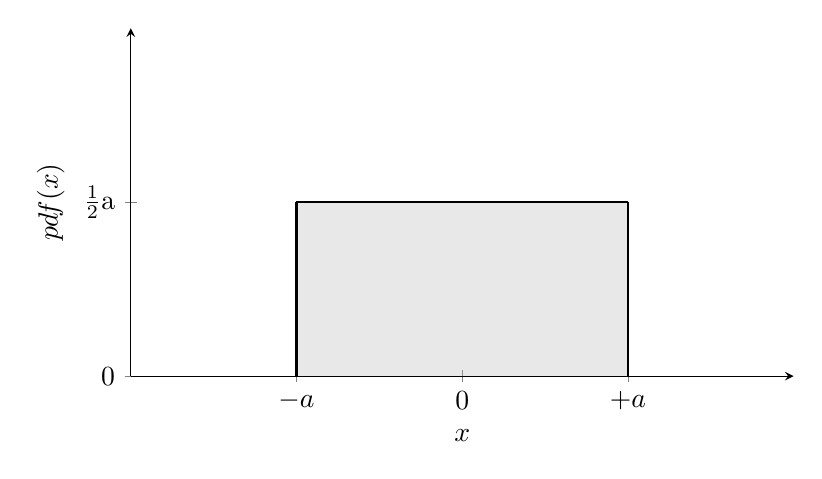
\begin{tikzpicture}
        \begin{axis}[
            clip=false,
            axis lines = left,
            xlabel = \(x\),
            ylabel = {\(pdf(x)\)},
            xmin = -2, xmax = 2,
            ymin = 0, ymax = 1,
            xtick = {-1, 0, 1},
            xticklabels = {$-a$, $0$, $+a$},
            ytick = {0, 0.5},
            yticklabels = {$0$, $\frac{1}{2}$a},
            width=10cm,
            height=6cm,
            domain=-2:2
        ]
        
        % Area evidenziata (distribuzione uniforme)
        \addplot [
            gray!30,
            fill=gray!60,
            opacity=0.3
        ] coordinates {
            (-1,0)
            (-1,0.5)
            (1,0.5)
            (1,0)
        };
    
        % Linea superiore della pdf
        \addplot [
            thick,
            black
        ] coordinates {
            (-1,0.5)
            (1,0.5)
        };
    
        % Linee verticali
        \addplot[thick] coordinates {(-1,0) (-1,0.5)};
        \addplot[thick] coordinates {(1,0) (1,0.5)};
    
        \end{axis}
    \end{tikzpicture}
    \end{center}
    
Considerando z il generico scostante in tale intervallo, si ha:

{
    \Large
    \begin{equation}
        p(z) = \frac{1}{2a}
    \end{equation}
}

p(z) è uguale a $\frac{1}{2a}$ proprio perchè, dall'esame di Teoria dei Segnali, l'area, 
cioè l'integrale della pdf deve essere uguale a uno. \newline 

Sapendo p(z) si può calcolare la varianza della misura x come: 

{
    \Large 
    \begin{equation}
        \begin{split}
            u^{2} (x)
            &= 
            \int_{-a}^{+a} 
            z^{2} p(z) dz 
            \\
            &= 
            \int_{-a}^{+a}
            z^{2} \frac{1}{2a} dz 
            \\ 
            &= 
            \frac{1}{2a} \cdot 
            \left.
                \frac{z^{3}}{3}
            \right|^{+a}_{-a}
            \\
            &= 
            \frac{a^{2}}{3}
        \end{split}
    \end{equation}
} 

Sapendo la relazione tra varianza e incertezza di tipo B, 
l'incertezza assoluta di tipo B associata alla quantità x risulta quindi: 

{
    \Large 
    \begin{equation}
        u(x) = \frac{a}{\sqrt{3}}
    \end{equation}
}


L'ipotesi di distribuzione uniforme è piuttosto pessimistica, ma è anche quella suggerita dalla GUM in mancanza di ulteriori informazioni. \newline 

Se invece possiamo ipotizzare che i valori centrali dell'intervallo [-a, +a] sono più probabili di verificarsi, 
si può assumere una distribuzione di tipo gaussiano, come in figura: 


\begin{figure}[h]
    \centering
    \includegraphics[scale = 0.4]{curva standard normalizzata di gaus.png}
\end{figure}

Se si considera: 

{
    \Large 
    \begin{equation}
        a = 3\sigma
    \end{equation}
}

si svolge il calcolo della varianza come abbiamo svolto per la distribuzione uniforme, 
ma, in questo caso, l'incertezza associata alla quantità x risulta in una distribuzione di tipo gaussiano come: 

{
    \Large
    \begin{equation}
        u(x) = \frac{a}{3}
    \end{equation}
}

Quindi, p(z) con distribuzione gaussiana è quella con l'incertezza più bassa possibile, 
invece p(z) con distribuzione costante è quella con l'incertezza più alta possibile. \newline 

\newpage 

\subsection{Distribuzione triangolare}
\footnote{Slide della prof | SDME 2 Incertezza secondo GUM parte II | pag 11 \\  
Appunti | 2025-03-11 | pag 4 - 5}

Un caso intermedio tra la distribuzione gaussiana e quella uniforme è quella triangolare: 

\begin{figure}[h]
    \centering
    \includegraphics[scale = 0.4]{Distribuzione di probabilità di tipo triangolare.png}
\end{figure}

in cui (tralascio i conti qui, ma il procedimento è lo stesso di prima):

{
    \Large 
    \begin{equation}
        u(x) = \frac{a}{\sqrt{6}}
    \end{equation}
}

\newpage 

\section{Incertezza combinata standard}
\footnote{Slide della prof | SDME 2 Incertezza secondo GUM parte II | pag 20 \\  
Appunti | 2025-03-11 | pag 5}

Quando si vuole svolgere una misura, 
si possono avere due situazioni limite: 

\begin{itemize}
    \item Singola misurazione, non è possibile stimare le incertezze di tipo A, si considerano unicamente quelle di tipo B 
    \item Infinite misurazioni, tutte le grandezze di influenza vengono fatte variare in modo casuale per stimare le cause di incertezza unicamente tramite metodo A
\end{itemize}

Essendo situazioni limite, sono situazioni che sono molto rare: allora, in tutte le misure, ci ritroveremo nel caso intermedio, 
quindi useremo i contributi di incertezza combinata standard. \newline

In genere, i contributi dell'incertezza combinata standard sono ottenuti tramite i metodi A e B contemporaneamente. \newline 



Stimati i contributi sia di tipo A che di tipo B, si passa al calcolo dell'incertezza combinata standard come: 

{
    \Large 
    \begin{equation}
        \begin{split}
        u_c (x)
        &= 
        \sqrt{\sum_{i = 1}^{N} u(x_i)^{2}}
        \\
        &= 
        \sqrt{(u_a (x))^{2} + (u_b (x))^{2} }
        \end{split}
    \end{equation}
}

Di seguito, si può calcolare il valore dell'incertezza estesa U(x) come: 

{ 
    \Large 
    \begin{equation}
        U (x) = k \cdot u_c (x)
    \end{equation}
}

dove k è il fattore di copertura che è un numero scelto intero, 
che tipicamente è compreso tra 1 e 3. \newline 

\newpage 

\section{Incertezza estesa}
\footnote{Slide della prof | SDME 2 Incertezza secondo GUM parte II | pag 18 - 19 \\  
Appunti | 2025-03-11 | pag 5 - 6}

L'incertezza composta $u_c (y)$ viene universalmente accettata per esprimere l'incertezza di una misurazione. \newline 

Normalmente, tuttavia, si richiede che la valutazione quantitativa dell'incertezza venga data come un intervallo U intorno al risultato della misurazione, 
che comprenda "ragionevoli" valori del misurando. \newline 

Da un punto di vista grafico, possiamo vedere il tutto come: 

\begin{figure}[h]
    \centering
    \includegraphics[scale = 0.6]{Incertezza estesa con note.PNG}
\end{figure}

Tale intervallo è denominato come incertezza estesa, 
e si ottiene moltiplicando l'incertezza composta $u_c (y)$ per un fattore di copertura. \newline 

In formule: 

{
    \Large 
    \begin{equation}
        U = k \cdot u_c (y)
    \end{equation}
}

Il fattore di copertura k viene scelto in base al livello di fiducia p che viene 
richiesto all'intervallo [(y - U) ÷ (y + U)]. \newline 

Il livello di fiducia p rappresenta la probabilità di copertura di questo intervallo, 
cioè la probabilità che il risultato dichiarato casa entro l'intervallo [(y - U) ÷ (y + U)]. \newline 

Il legame fra k e p può essere stabilito se sono note le distribuzioni di probabilità 
che caratterizzano i risultati della misurazioni. \newline 

In genere, quindi, non è facile determinare un legame rigoroso. \newline 

Nella pratica, si può ritenere che: 

\begin{itemize}
    \item k = 2, corrisponda a un livello di fiducia di circa il 95 \% 
    \item k = 3, corrisponda a un livello di fiducia di circa il 99 \%
\end{itemize}

\newpage 

\section{Combinazione delle incertezze}
\footnote{Slide della prof | SDME 2 Incertezza secondo GUM parte II | pag 12 - 17 \\  
Appunti | 2025-03-11 | pag 7 - 9}

La GUM si basa su principi lineari e distribuzioni gaussiane, ma, se il fenomeno non lo è, 
la GUM offre degli appendici riguardo al caso non lineare e/o con distribuzioni non gaussiane. \newline 

In questo corso, ci concentriamo solo su principi lineari e distribuzioni gaussiane. \newline 

La definizione dello scarto tipo o della varianza si rivela particolarmente utile nell'analisi 
della combinazione delle incertezze di più fenomeni aleatori, 
cioè nella valutazione dell'incertezza di quantità determinate in modo indiretto: 

{ 
    \Large 
    \begin{equation}
        y = f(x_1, x_2, ..., x_m)
    \end{equation}
}

dove $x_i \text{ } (i = 1, ..., m)$ viene considerata una variabile aleatoria di una grandezza indipendente. \newline 

Si dimostra (cioè non lo dimostriamo) che, se le variabili aleatorie sono tutte fra loro statisticamente indipendenti, 
l'incertezza stimata sulla determinazione indiretta della quantità y, risulta: 

{
    \Large 
    \begin{equation}
        u_c (y) = \sqrt{\sum_{i = 1}^{m} \left[ \left( \frac{\partial f}{\partial x_i} \right) ^{2} u^{2} (x_i)\right]}
    \end{equation}
}

dove 

\begin{itemize}
    \item $u_c (y)$ è l'incertezza tipo composta associata alla grandezza y 
    \item $\frac{\partial f}{\partial x_i}$ è chiamato coefficiente di sensibilità
\end{itemize}

\begin{tcolorbox}
    La frazione $\frac{\partial f}{\partial x_i}$ può, inizialmente, far paura; la si può vedere in questa maniera: \\
    essendo f una funzione di m variabili, fare la derivata parziale della grandezza $x_i$ è come esprimere quanto influisce la grandezza $x_i$ su tutte le altre m-1 grandezze 
    se le m-1 grandezze rimangono costanti
\end{tcolorbox}

Inoltre, in presenza di correlazione fra le variabili di ingresso, 
$u_c (y)$ si può esprimere come: 

{
    \Large 
    \begin{equation}
        u_c (y) = \sqrt{\sum_{i = 1}^{m} \left[ \left( \frac{\partial f}{\partial x_i} \right) ^{2} u^{2} (x_i)\right]
        2 \sum_{i=1}^{m-1} \sum_{j = i+1}^{m}
        \frac{\partial f}{\partial x_i}
        \frac{\partial f}{\partial x_j}
        cov (x_i, x_j)        
        }        
    \end{equation}
}

dove con $cov(x_i, x_j)$ rappresenta la covarianza tra le due variabili e quindi della loro mutua indipendenza. \newline 

La covarianza $cov(x_i, x_j)$ può essere sia positiva che negativa, quindi può comportare sia incrementi che riduzioni dell'incertezza composta $u_c (y)$. \newline 

\begin{tcolorbox}
    Questa ultima formula di $u_c (y)$ NON la useremo mai nel corso perchè, dalla Teoria dei segnali, confideremo le grandezze statisticamente indipendenti, 
    quindi la $cov (x_i, x_j)  = 0$. \newline 

    Perché ho scritto questa formula? Perché la prof ha detto a lezione che la dobbiamo sapere. Fine
\end{tcolorbox}

Di seguito, delle tabelle riassuntive per le leggi di propagazione per legami funzionali semplici: 

\begin{figure}[h]
    \centering
    \includegraphics[scale = 0.3]{leggi di propagazione per legami funzionali semplici.PNG}
    \includegraphics[scale = 0.3]{leggi di propagazione per legami funzionali semplici 2.PNG}
\end{figure}

\newpage

L'equazione per il calcolo di $u_c$ è spesso chiamata come legge di propagazione delle incertezze, 
ed è di grande utilità nella valutazione di incertezze per grandezze misurate per via indiretta. \newline 

La GUM consiglia, se possibile, di fare sempre misure dirette, ma, se ciò non è possibile, possiamo utilizzare queste relazioni. \newline 

Quando la funzione f non è definita e/o è difficile esplicitarla, si impiegano altri metodi alternativi, come ad esempio le simulazioni. \newline 

\newpage

\section{Supplemento GUM: simulazione Monte Carlo}
\footnote{Slide della prof | SDME 2 Incertezza secondo GUM parte II | pag 22 - 33 \\  
Appunti | 2025-03-05 | pag 9 - 10 | 2025-03-12 | pag 2 - 5}

\begin{tcolorbox}
    Questa sezione non la dobbiamo sapere bene e nel dettaglio come le altre: è un qualcosa in più
\end{tcolorbox}

Se la funzione tra le varie grandezze non è nota in maniera analitica e/o completa, il supplemento della GUM (il JCGM 101:2008) 
consiglia di implementare la simulazione Monte Carlo per il calcolo  delle propagazioni. \newline 

La simulazione Monte Carlo (in generale tutte le simulazioni perchè impiegano tempo e risorse) va utilizzata se: 

\begin{itemize}
    \item il modello funzionale devia fortemente dalla linearità 
    \item le derivate parziali sono difficilmente calcolabili 
    \item le distribuzioni di probabilità associate alle grandezze da misurare non sono gaussiane 
    \item la propagazione delle incertezze fornisce una sovrastima dell'incertezza associata alla misura finale 
    \item modello funzionale non completamente noto 
    \item modello funzionale complicato
\end{itemize}

Per la simulazione Monte Carlo si sceglie almeno un numero di $10^{6}$ simulazioni. \newline 

\newpage 

\section{Esprimere l'incertezza}
\footnote{Slide della prof | SDME 2 Incertezza secondo GUM parte II | pag 34 \\  
Appunti | 2025-03-12 | pag 5 - 6}

Possiamo riassumere tutto questo capitolo con i seguenti passaggi. \newline 

Di seguito, l'algoritmo step-by-step per esprimere l'incertezza di una misura: 

\begin{enumerate}
    \item Descrivere chiaramente il metodo usato per calcolare il risultato della misura e l'incertezza correlata 
    \item  Riportare una lista contenente tutte le componenti dell'incertezza e come esse sono state calcolate 
    \item Nel caso di incertezza estesa $U(x) = k \cdot u_c (x)$ occorre: 
    \begin{itemize}
        \item Fornire una descrizione esaustiva di come il parametro è definito 
        \item Riportare il risultato della misurazione come $X = x \pm U$ fornendo l'unità di misura 
        \item Fornire l'incertezza estesa relativa $U / \abs{x}$ 
        \item Riportare il valore di k 
        \item Fornire il livello di confidenza approssimato associato con l'intervallo $x \pm U$ e come è stato calcolato
    \end{itemize}
    \item Se si misurano due grandezze contemporaneamente, oltre alla misura e alle incertezze relative ad ogni parametro, bisogna fornire la covarianza ed il coefficiente di correlazione
\end{enumerate}

\begin{tcolorbox}
    L'ultimo punto riguardo la covarianza è vero in generale per tutte le misure, ma, come ho scritto precedentemente, in questo corso consideriamo grandezze indipendenti 
    in cui la covarianza è nulla. \newline 

    Si, in questo corso scriverò più e più volte le stesse cose, è un po' come andare a lezione: \\ 
    repetita iuvant , dicevano i romani
\end{tcolorbox}

\newpage 

